In this section, the processing layer's hardware and software design are delineated. The layer comprises a PLC, Raspberry Pi, and a PC interconnected to facilitate communication and decision-making processes. The PLC primarily governs the robotic arm's movements, including all joints and an additional axis, typically a linear rail. Conversely, the Raspberry Pi is tasked with data collection and transmission to the PC for decision-making regarding task execution on incoming objects, typically boxes. Communication between the PC and PLC ensures alignment of all arm joints for task performance. This section delves into implementation details, covering hardware components, programming languages, software dependencies, and operating systems relevant to the processing layer. Unnecessary details, such as purely software modules without specific hardware components, are omitted for conciseness. Adjustments to the organization, titles, and content are permissible to suit the project's requirements.


\subsection{Layer Hardware}
The hardware involved with the processing layer include a MELSEC Programmable Logic Controller, issued by Mitsubishi. The PLC is a specialized computer used in industrial automation and is paired with software to make decisions based on sensor data like temperature, pressure, or motor position. Finally, the PLC is equipped with an ethernet switch that enables communication between the Host PC and PLC.
\subsection{Layer Operating System}
The operating systems required by the layer are dependent on the specific components. The PLC runs a real-time operating system (RTOS), while the Raspberry Pi utilizes a Linux-based operating system Raspbian, and the host PC runs Windows 10.


\subsection{Layer Software Dependencies}
There are currently no software dependencies.
\subsection{Host PC}
The host PC acts as a powerful processing unit for in-depth analysis, decision making, and control. It receives pre-processed data from the Raspberry Pi, including data from the QR code, and it performs trajectory planning and higher level decision making.

\begin{figure}[h!]
	\centering
 	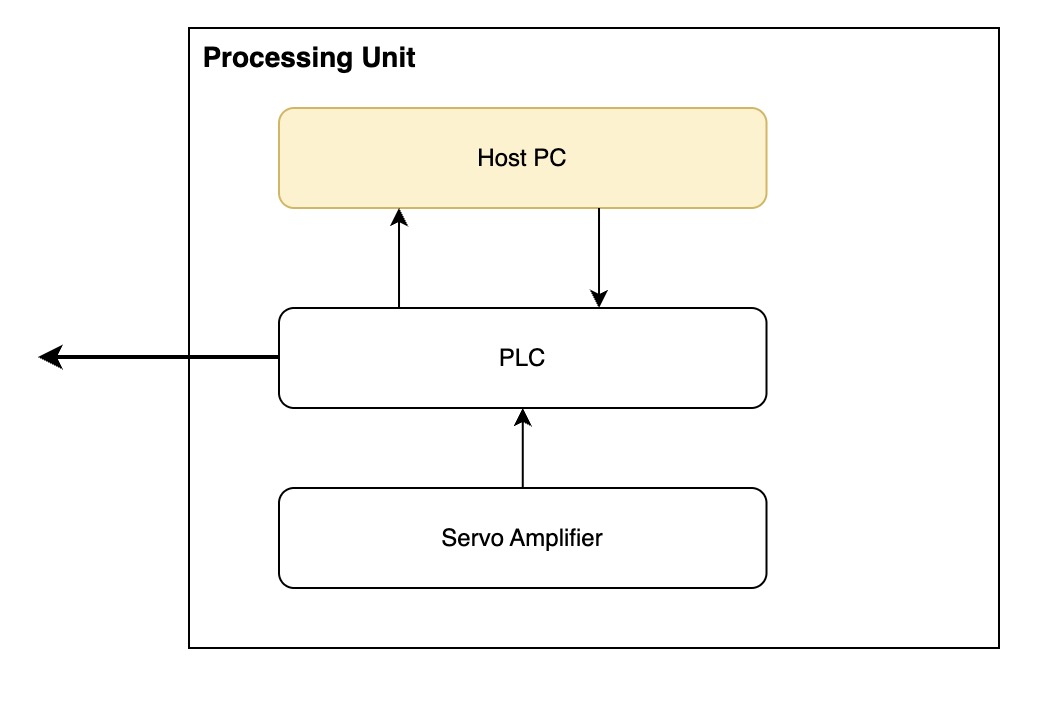
\includegraphics[width=0.6\textwidth]{images/HostPC.jpg}
 \caption{Host PC Subsystem}
\end{figure}

\subsubsection{Subsystem Hardware}
This subsystem consists of a Dell desktop computer with USB connections to the RV-8CRL controller. 
\subsubsection{Subsystem Operating System}
The PC runs Windows 10.
\subsubsection{Subsystem Software Dependencies}
The PC runs several software for the system including RT ToolBox3, GXWorks, MRConfigurator2, and Creality.
\begin{itemize}
    \item RT ToolBox is a software developed by Mitsubishi used for visual programming of the robotic arm, acting as a 3D simulator.
    \item GXWorks is a software suite provided by Mitsubishi Electric for programming and configuring PLCs. It is a comprehensive development environment that supports various programming languages such as ladder logic, function block diagrams (FBD), and structured text (ST).
    \item MRConfigurator2 is a software tool used for programmign Mitsubishi's servo drives and motion controllers.
    \item Creality is used for 3D modeling and design. Primarily, this software is used for designing mechanical components.
\end{itemize}

\subsubsection{Subsystem Programming Languages}
The Host PC uses Python scripts for network communication. The RT ToolBox software supports MELFA-BASIC-VI programming language.

\subsubsection{Subsystem Data Processing}
Upon receiving preprocessed data from the Raspberry Pi, the Host PC engages in thorough data analysis. This includes examining sensor data performing image processing if necessary. Algorithms for noise reduction, edge detection, and image segmentation may be employed to extract relevant information from sensor readings or images. The Host PC manages communication with the PLC using Ethernet/IP. Data packets are assembled and parsed according to the protocol specifications, ensuring reliable and efficient data exchange between the PC and the PLC.

\subsection{Additional Axis Servo}
This subsystem focuses on controlling the additional axis, such as a linear rail, to facilitate precise movements of the robotic arm.
\begin{figure}[h!]
	\centering
 	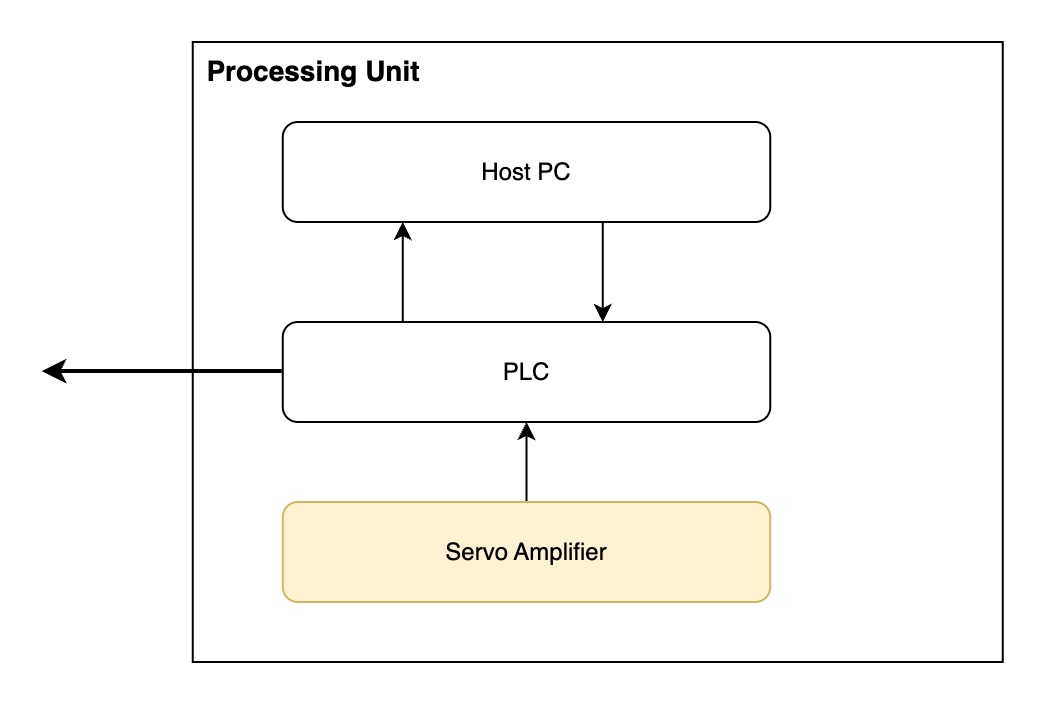
\includegraphics[width=0.65\textwidth]{images/ServoAmp.jpg}
 \caption{Servo Subsystem}
\end{figure}

\subsubsection{Subsystem Hardware}
The subsystem consists of a RollOn linear axis on a Megadyne belt. The servo amplifier is a MELSERVO MR-J4 series. Connections between the servo amplifier and PLC occur through a USB-A.
\subsubsection{Subsystem Software Dependencies}
Servo amplifier parameters are dependent on MRConfigurator2, where they can be specified through read/write operations.

\subsubsection{Subsystem Data Processing}
The servo amplifier receives control signals from the controller and translates them into precise voltage and current outputs to drive a servo motor. It continuously monitors feedback from sensors to maintain accurate motor position and velocity, adjusting operation as needed to minimize discrepancies. Additionally, servo amplifiers incorporate safety features to prevent damage and ensure safe operation of the motor system.


\subsection{Programmable Logic Controller}
The PLC acts as the central component of the processing layer, responsible for coordinating and executing control tasks for the robotic arm and additional axis. This subsection outlines the hardware, software, and data processing aspects specific to the PLC.
\begin{figure}[h!]
	\centering
 	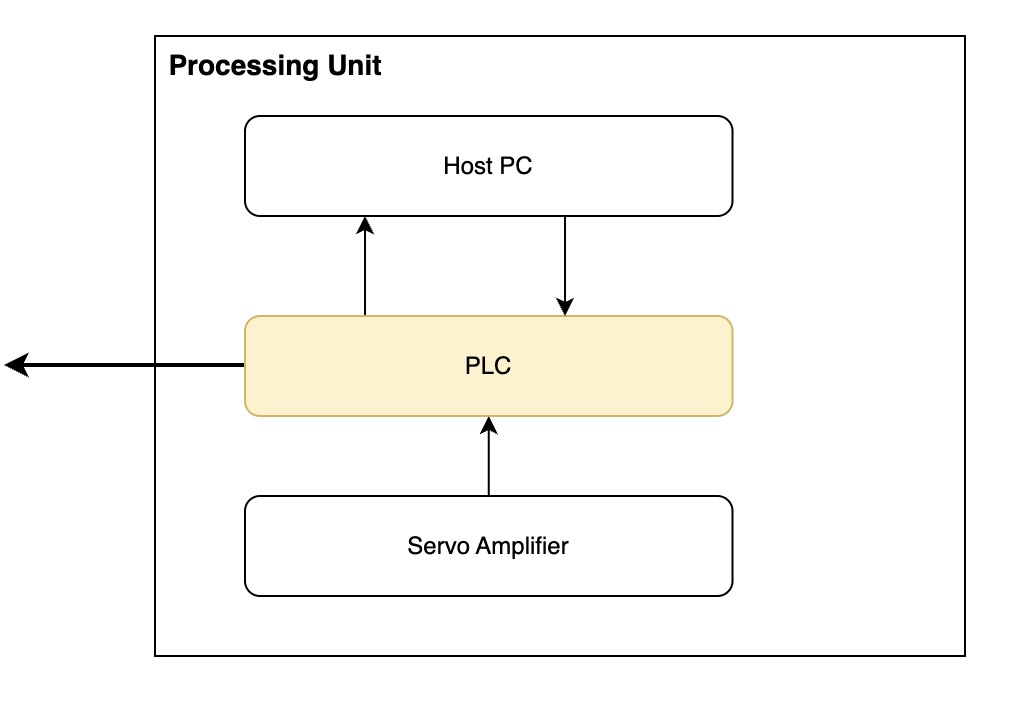
\includegraphics[width=0.65\textwidth]{images/PLC.jpg}
 \caption{PLC Subsystem}
\end{figure}

\subsubsection{Subsystem Hardware}
The PLC consists of a MELSEC Programmable Logic Controller manufactured by Mitsubishi, equipped with an integrated ethernet switch for communication with the host PC.

\subsubsection{Subsystem Operating System}
Operating on a real-time operating system (RTOS), the PLC ensures precise timing and reliable execution of control logic.

\subsubsection{Subsystem Software Dependencies}
Software tools such as GXWorks and MRConfigurator2, provided by Mitsubishi Electric, enable the programming and configuration of the PLC for control tasks.


\subsubsection{Subsystem Programming Languages}
Programming languages supported by GXWorks, including ladder logic, function block diagrams, and structured text, are utilized for developing control algorithms tailored to the application. RT ToolBox is written in MELFA BASIC VI


\subsubsection{Subsystem Data Processing}
The PLC processes sensor feedback and command signals in real-time, executing control logic to coordinate the movements of the robotic arm and additional axis. Communication with the host PC via Ethernet/IP facilitates efficient data exchange for seamless system operation.









